%!TEX root = ../NeuralNets.tex
\section{Boltzmann Machines}\label{sec:bm}\xindex{Boltzmann Machine}%
Literature: \cite{Bengio2009}

\emph{Boltzmann machines} are stochastic recurrent neural networks. They work similar \emph{Hopfield nets} in that they have a binary state vector ($s_j \in {0,1}$), which is sometimes divided in visible states (neurons) $v_j$ and hidden neurons $h_j$. But while the activation calculation in \emph{Hopfield nets} is deterministically, it is stochastic for \gls{BM}.

\begin{equation}
z_j = b_j + \sum_i v_i w_{ij}
\end{equation}
The probability that the activation of neuron $s_j$ is set to $1$ is calculated using the sigmoid function,
\begin{equation}
p(s_j = 1) = \sigma(v_j) = \frac{1}{1 + e^{-z_j}}
\end{equation}
, otherwise the activation of $s_j$ becomes $0$.

Further we define the network architecture as follows
\begin{itemize}
\item Network is fully connected
\item No self connections, $w_{ii}=0$
\item Undirected/symmetric, $w_{ij}=w_{ji}$
\end{itemize}

\subsection{Energy-based models}
\todo{Derivations of energy-based models, see \cite{Bengio2009}}

% The energy of a state $v$ is defined by
% \begin{align}
% E(v) &= - \sum_i v_i b_i - \half \sum_{i,j} v_i v_j w_{ij}
% \intertext{and define our normalizing factor $Z$ as}
% Z &= \sum_u e^{-E(u)}
% \intertext{with loads as to our state probability}
% p(v) &= \frac{e^{-E(v)}}{\sum_u e^{-E(u)}} = \frac{e^{-E(v)}}{Z} \,.\label{eq:uiae}
% \end{align}

% So far all our neurons were visible neurons, to increase the computational power we will add hidden neurons $h_j$.
% \begin{align}
% p(v,h) &= \frac{e^{-E(v,h)}}{Z}
% \intertext{and because only the visible units $v_j$ are observed, we care about the marginal}
% p(v) &= \sum_h \frac{e^{-E(v, h)}}{Z}
% \end{align}

% To map this formulation to one similar to \cref{eq:uiae}, we introduce the notation of \emph{free energy} $F$:
% \begin{align}\label{eq:free-energy}
% F(v) &= - \log \sum_h e^{-E(v,h)} \\
% Z &= \sum_v e^{-F(v)} &= \sum_v e^{\log \sum_h e^{-E(v,h)}} &= \sum_v \sum_h e^{-E(v,h)}\\
% p(v) &= \frac{e^{-F(v)}}{Z} &= \frac{e^{\log \sum_h e^{-E(v,h)}}}{Z} &= \sum_h \frac{e^{-E(v,h)}}{Z}
% \end{align}

% So we just swifted everything to the $\log$ domain. This gives us the log-likelihood gradient.
% \begin{align}
% \frac{\partial \log p(v)}{\partial \theta}
% &= \frac{\partial F(v)}{\partial \theta} + \frac{1}{Z} \sum_u e^{-F(u)} \frac{F(u)}{\partial \theta}\\
% &= \frac{\partial F(v)}{\partial \theta} + \sum_u p(u) \frac{F(u)}{\partial \theta}\\
% \end{align}


\subsection{Energy of Boltzmann Machines}
\begin{align}\label{eq:bm-energy}
E(s) &= - \sum_i b_i s_i - \sum_{i,j} s_i w_{ij} s_j\\
E(v,h) &= - \sum_i b_i v_i - \sum_i c_i h_i - \sum_{i,j} v_i w_{ij}^{vh} h_j - \sum_{i,j} v_i w_{ij}^{vv} v_j - \sum_{i,j} h_i w_{ij}^{hh} h_j
\end{align}

\subsection{Training}
Training is done by calculating the gradient of the log-likelihood derived by
the the parameter set $\theta$.
\begin{equation}
\frac{\partial \log p(v)}{\partial \theta}
\end{equation}

\todo{Training of BMs}

\subsection{Simulated Annealing}
Use temperature $T$ to allow more changes in the beginning (\eg jumps out of bad local minima) by using the sigmoid function with $\beta=\frac{1}{T}$.
\begin{equation}
p(s_j = 1) = \frac{1}{1 + e^{\frac{-z_j}{T}}}
\end{equation}
\Cref{fig:bm-simulated-annealing} shows curves with different temperature.

\begin{figure}
\centering
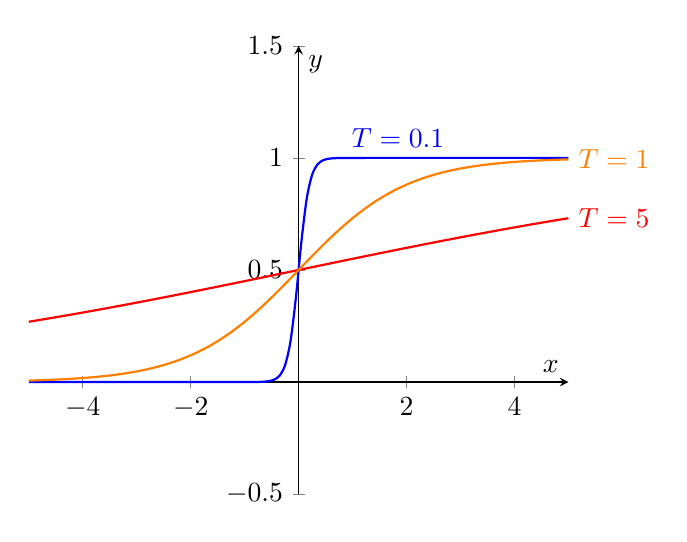
\begin{tikzpicture}
\begin{axis}[
	axis lines = middle,
	xlabel = $x$,
	ylabel = $y$,
	ymin = -0.5,
	ymax = 1.5,
	xmin = -5,
	xmax = 5,
	clip = false,
]
\addplot[
	samples = 100, 
	color = red,
	thick, smooth,
	]
{1/(1+e^(-x/5))}
node[right,pos=1] {$T=5$};
\addplot[
	samples = 100, 
	color = blue,
	thick, smooth,
	]
{1/(1+e^(-x/0.1))}
node[above,pos=0.7] {$T=0.1$};

\addplot[
	samples = 100, 
	color = orange,
	thick, smooth,
	]
{1/(1+e^(-x))}
node[right,pos=1] {$T=1$};
\end{axis}
\end{tikzpicture}
\caption{Sigmoid function (orange), with high temperature (red) and low temperature (blue).}
\label{fig:bm-simulated-annealing}
\end{figure}

\subsection{Why to restrict BMs}
Unrestricted Boltzmann machines are very powerful and can compute every
function. But due the complex net structure the training is very slow and
computational expensive. \Glspl{RBM} applying constraints to the network
architecture, but can still compute any function.


